If we instead approach DIS as the production and absorption of a virtual photon by a parton we can extract a different structure function $R=\sigma_L/\sigma_T$, referred to as photonuclear R. That is, the ratio of the cross sections for absorbing longitudinal photons, $\sigma_L$, to transverse photons, $\sigma_T$. In the Bjorken limit, as in the previous section, $R\rightarrow 0$. In practice the Bjorken limit is an imperfect approximation and it is useful to consider the effects of large, but finite, $Q^2$ and $\nu$.

We can write the DIS cross section in terms of these cross sections as
\begin{equation}
	\frac{d^2\sigma}{d\Omega dE^\prime}\left(E,E^\prime,\theta\right) = \Gamma\left[\sigma_T\left(x,Q^2\right)+\epsilon\sigma_L\left(x,Q^2\right)\right].
\end{equation}
In this equation $\Gamma$ is the flux of transverse virtual photons and $\epsilon$ is the relative flux of longitudinal virtual photons. These are defined by
\begin{equation}
	\Gamma = \frac{\alpha KE^\prime}{2\pi^2Q^2E_0\left(1-\epsilon\right)}
\end{equation}
and
\begin{equation}
	\epsilon = \frac{1}{1+2\left(1+\nu^2/Q^2\right)\tan^2\left(\frac{\theta}{2}\right)}.
\end{equation}
Here, $K$ is the laboratory photon energy,
\begin{equation}
	K = \frac{W^2-M^2}{2M}.
\end{equation}

By comparing these equations to Equation \ref{eqn:x_dis_xs} $F_1$ and $F_2$ can be related to $\sigma_L$, $\sigma_T$, and each other.

\begin{equation}
	\sigma_T = \frac{4\pi\alpha^2}{KM} F_1
\end{equation}

\begin{equation}
	\sigma_L = \frac{4\pi\alpha^2}{KM}\frac{1}{2x}\left[F_2 - 2xF_1\right]
\end{equation}

\begin{equation}
	F_1 = \frac{F_2\left(1+Q^2/\nu^2\right)}{2x\left(1+R\right)}
\end{equation}

Substituting this into our DIS cross section equation, we can eliminate $F_1$. This also makes it clear that we can easily access the $F_2$ structure functions by measuring cross section ratios.

\begin{equation}
	\frac{d^2\sigma}{d\Omega dE^\prime}\left(E,E^\prime,\theta\right) = \frac{4\alpha^2\left(E^\prime\right)}{Q^4}\cos^2\left(\frac{\theta}{2}\right)F_2\left[\frac{1}{\nu}+\frac{\left(1+Q^2/\nu^2\right)}{xM\left(1+R\right)}\tan^2\left(\frac{\theta}{2}\right)\right]
\end{equation}

If we measure the cross section ratios of two different targets at the same kinematics (that is the same $x$, $E$, $E^\prime$, and $\theta$) we find:

\begin{equation}
	\frac{\sigma_A}{\sigma_B} = \frac{F_2^A}{F_2^B} \frac{\left[\frac{1}{\nu}+\frac{\left(1+Q^2/\nu^2\right)}{xM\left(1+R^A\right)}\tan^2\left(\frac{\theta}{2}\right)\right]}{\left[\frac{1}{\nu}+\frac{\left(1+Q^2/\nu^2\right)}{xM\left(1+R^B\right)}\tan^2\left(\frac{\theta}{2}\right)\right]}
\end{equation}

As shown in Figure \ref{R_no_A}, historical data suggests that photonuclear R has no nuclear dependence to within $10\%$. If we assume that that there is no nuclear dependence, this equation simplifies to:

\begin{figure}
\begin{center}
	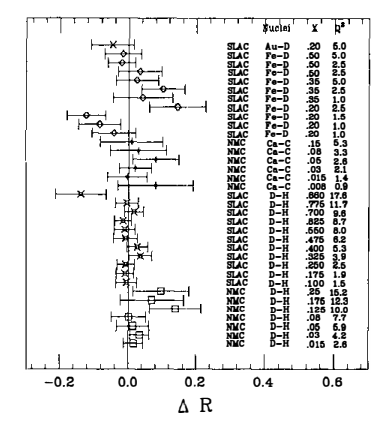
\includegraphics{./scattering/fig/R_LT.png}
	\caption{Historical data of $R=\sigma_L/\sigma_T$. This data shows measurements of the difference in $R$ between two nuclei. The data is consistent with no nuclear dependence.\cite{GST}}
	\label{R_no_A}
\end{center}
\end{figure}

\begin{equation}
	\frac{\sigma_A}{\sigma_B} = \frac{F_2^A}{F_2^B}
\end{equation}

By measuring the cross section ratios of targets in the DIS region, we can easily access the nuclear structure functions of the targets.